\chapter{Detección de áreas inundadas}

Esta clase tiene como objetivo aplicar los conceptos estudiados durante el curso, para la detección se espejos de agua, utilizando imágenes \emph{Sentinel 1}. Se trabajrá con las inundaciones de octubre de 2017 en la zona de Chascomús, provincia de Buenos Aires, Argentina.

% Imagen antes
% S1B_IW_GRDH_1SDV_20171007T090618_20171007T090643_007721_00DA33_E6D1

% Subset
% N = -35.632
% W = -57.395
% S = -35.933
% E = -58.569

\section{Actividades}

\begin{que}
    Descargue la imagen del 10 de octubre del 2017
    \begin{center}\path{ S1B_IW_GRDH_1SDV_20171007T090618_20171007T090643_007721_00DA33_E6D1}\end{center} del \href{https://vertex.daac.asf.alaska.edu/}{Alaska Satellite Facility}. Utilice la búsqueda por \emph{Granule} en lugar de la \emph{Geospatial}.
\end{que}

\begin{que}
    Con la herramienta \menu{Raster>Subset} (Figura \ref{fig:coordenadas}) haga un recorte entre las coordenadas geográficas
    \begin{figure}[h!]
        \centering
        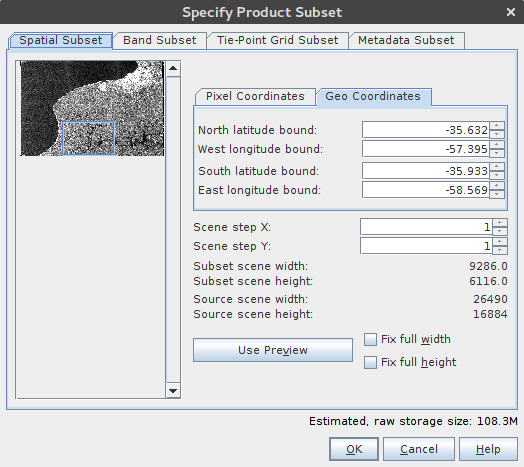
\includegraphics[scale=0.4]{fig:coordenadas.png}
        \caption{}
        \label{fig:coordenadas}
    \end{figure}
    \begin{itemize}
        \item Latitud norte: -35.632
        \item Longitud oeste: -57.395
        \item Latitud sur: -35.933
        \item Longitud este: -58.569
    \end{itemize}


\end{que}

\begin{que}
    Procese la imagen como se realizó en la clase 3. Calíbrela para obtener el coeficiente de backscatter, aplique los filtros correspondientes y proyectela en terreno utilizando un DEM. Exporte la vista obtenida en dB.
\end{que}

\begin{que}
    En la imagen, identifique cuerpos de agua, vegetación y ciudades. Mida su coeficiente de retrodispersión en las bandas VV y VH. Seleccione que polarización separa mejor las zonas con y sin agua.
\end{que}

\begin{que}
    Utilizando la herramienta \menu{Analysis>Histogram} calcule el histograma de la imagen e identifique un valor por debajo del cual, el coeficiente de retrodispersión corresponde a agua.
\end{que}

\begin{que}
    Obtenga un mapa de zonas anegadas. Seleccione la herramienta \menu{Band maths...} (Figura \ref{fig:bm}) con click derecho sobre el nombre de la imagen e ingrese la formula
    \begin{center}
        \path{BANDA < T}
    \end{center}
    donde T es el valor obtenido en el punto anterior.
    \begin{figure}[h!]
        \centering
        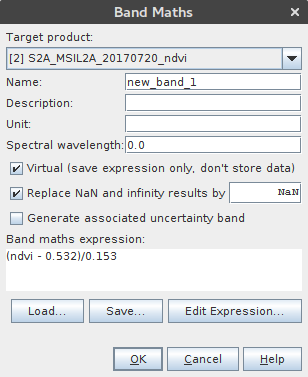
\includegraphics[scale=0.4]{fig:bm.png}
        \caption{}
        \label{fig:bm}
    \end{figure}
\end{que}

\begin{que}
    Exporte el mapa como KMZ.
\end{que}

\begin{que}
    Repita el proceso para la imagen del 30 de septiembre de 2016
    \begin{center}
        \path{S1B_IW_GRDH_1SDV_20160930T090612_20160930T090637_002296_003E21_85E2}
      
\end{que}

\begin{que}
    Compare las zonas inundadas en 2016 y 2017.
\end{que}
